\documentclass[10pt,letterpaper,twocolumn]{article}

\usepackage[utf8]{inputenc}
\usepackage[T1]{fontenc}
\usepackage{mathptmx}
\usepackage{geometry}
\usepackage{graphicx}
\usepackage{amsmath}
\usepackage{booktabs}
\usepackage{array}
\usepackage{caption}
\usepackage{titlesec}
\usepackage{cite}
\usepackage{url}
\usepackage{balance}

\geometry{
  letterpaper,
  top=1in,
  bottom=1.125in,
  left=0.8125in,
  right=0.8125in
}
\setlength{\columnsep}{0.3125in}
\setlength{\parindent}{0.1667in}
\setlength{\parskip}{0pt}
\pagestyle{empty}

\renewcommand{\thesection}{\Roman{section}}
\renewcommand{\thesubsection}{\Alph{subsection}}

\titleformat{\section}
  {\normalfont\centering\scshape}
  {\thesection.}{0.5em}{}
\titleformat{\subsection}
  {\normalfont\itshape}
  {\thesubsection.}{0.5em}{}
\titlespacing*{\section}{0pt}{1.0ex plus 0.2ex minus 0.2ex}{0.6ex}
\titlespacing*{\subsection}{0pt}{0.8ex plus 0.2ex minus 0.2ex}{0.4ex}

\DeclareCaptionLabelFormat{procommfigure}{\textsc{Figure~#2.}}
\DeclareCaptionLabelFormat{procommtable}{\textsc{Table~#2}}
\captionsetup[figure]{
  font=small,
  labelformat=procommfigure,
  justification=raggedright,
  singlelinecheck=false
}
\captionsetup[table]{
  font=small,
  labelformat=procommtable,
  textfont=sc,
  justification=centering,
  singlelinecheck=false,
  position=top
}

\begin{document}
\twocolumn[
\begin{@twocolumnfalse}
\begin{center}
{\fontsize{24}{28}\selectfont Machine Learning-Based Weather Condition Classification with Leakage-Aware Preprocessing and Comparative Model Evaluation\par}
\vspace{0.8em}
{\fontsize{12}{14}\selectfont
M. Komal Narasimha Rao\\
Roll No. 251LA18011\\
komalnarashimharao@gmail.com
\par}
\end{center}

\vspace{0.8em}
\noindent\textbf{\textit{Abstract}}---Weather condition classification can support downstream planning tasks, but heterogeneous meteorological variables and imbalanced label distributions make the modeling pipeline sensitive to preprocessing choices. This paper reports a comparative machine-learning experiment conducted on the Kaggle Weather Dataset, comprising 96{,}453 hourly records with summary labels and meteorological measurements. The workflow preserves \textit{Summary} strictly as the prediction target and excludes it from all input transformations to avoid target leakage. Preprocessing removes non-informative fields, derives calendar attributes from the timestamp, converts wind bearing into sine and cosine components, imputes missing numerical and categorical values, standardizes numerical variables with z-score scaling, and one-hot encodes precipitation type. Because three classes had only one observation each, they were removed before stratified splitting. Logistic Regression, Decision Tree, and Random Forest classifiers were trained using an 80/20 stratified train-test split with \textit{random\_state} 42 and evaluated with weighted accuracy, precision, recall, and F1-score. Random Forest was selected as the best model by weighted F1-score, achieving 0.6215 accuracy, 0.6374 precision, 0.6215 recall, and 0.6175 F1-score. The results indicate that ensemble tree learning handles nonlinear feature interactions and class overlap more effectively than the linear and single-tree baselines in this dataset.

\vspace{0.5em}
\noindent\textbf{\textit{Index Terms}}---classification, machine learning, meteorological data, weather prediction
\vspace{1.0em}
\end{@twocolumnfalse}
]

\section{Introduction}
Weather condition prediction is important for transportation planning, agriculture, energy management, and risk awareness because atmospheric variables change continuously and interact in nonlinear ways. Data-driven weather analytics has therefore become a practical complement to traditional forecasting workflows, especially for localized classification tasks based on observed meteorological measurements \cite{zhang2025survey, chen2023survey}. Even in comparatively simple supervised-learning settings, however, weather datasets combine numerical, temporal, and categorical variables whose scales, cyclic behavior, and class imbalance can affect model behavior.

This study examines a weather-condition classification pipeline built on the Kaggle Weather Dataset \cite{kaggleweather}. The experiment focuses on predicting the label \textit{Summary} from processed meteorological features while explicitly preventing target leakage by excluding \textit{Summary} from all feature transformations. The workflow also addresses practical issues that arise in applied machine learning, including timestamp decomposition, circular wind-direction encoding, category handling, standardization, and extremely rare classes.

The contributions of the paper are modest but concrete. First, it documents a leakage-aware preprocessing pipeline for heterogeneous weather observations. Second, it compares Logistic Regression, Decision Tree, and Random Forest classifiers under a common stratified evaluation protocol. Third, it analyzes the observed performance differences using the actual saved outputs of the experiment, including class distribution, confusion-matrix structure, and Random Forest feature importance.




\section{Dataset and Preprocessing}
\subsection{Dataset Description}
The experiment uses the Kaggle Weather Dataset \cite{kaggleweather}. The raw file contains 96{,}453 hourly records and 12 original attributes: \textit{Formatted Date}, \textit{Summary}, \textit{Precip Type}, \textit{Temperature (C)}, \textit{Apparent Temperature (C)}, \textit{Humidity}, \textit{Wind Speed (km/h)}, \textit{Wind Bearing (degrees)}, \textit{Visibility (km)}, \textit{Loud Cover}, \textit{Pressure (millibars)}, and \textit{Daily Summary}. The modeling target is the multiclass weather label \textit{Summary}. This target was preserved for supervision and was not used as an input feature at any preprocessing stage.

After preprocessing, the saved normalized dataset contains 15 input features and the unchanged target column \textit{Summary}. The final processed columns are six meteorological measurements, five date-derived features, two wind-direction components, two one-hot precipitation indicators, and the target label.

\subsection{Data Cleaning}
The preprocessing notebook removes \textit{Loud Cover} because it is constant in the raw file and therefore non-informative for classification. It also drops \textit{Daily Summary}, which is a free-text descriptive field rather than a structured input variable for the chosen models. The raw CSV does not contain blank cells, but it includes 517 literal \texttt{null} entries in \textit{Precip Type}. For robustness, the pipeline applies median imputation to numerical features and most-frequent imputation to the categorical feature before model-ready transformation.

The processed dataset contains no missing values after transformation. This is consistent with the saved modeling input, where all 15 predictor columns are fully populated.

\subsection{Feature Engineering}
The field \textit{Formatted Date} is converted to a timezone-aware timestamp and decomposed into \textit{Year}, \textit{Month}, \textit{Day}, \textit{Hour}, and \textit{DayOfWeek}. This transformation allows the classifiers to access seasonal and intra-day patterns without retaining the original timestamp string.

Wind bearing is a circular variable, so the notebook replaces \textit{Wind Bearing (degrees)} with
\begin{equation}
\text{Wind Direction Sin} = \sin(\theta), \qquad
\text{Wind Direction Cos} = \cos(\theta),
\end{equation}
where $\theta$ is the wind-bearing angle in degrees after conversion to radians. This avoids the artificial discontinuity between angles near $0^\circ$ and $360^\circ$.

The only categorical predictor, \textit{Precip Type}, is one-hot encoded with unknown categories ignored at inference time. In the saved processed file, this produces the binary indicators \textit{Precip Type\_rain} and \textit{Precip Type\_snow}. Importantly, \textit{Summary} is not encoded as an input variable; it remains the output label only.

\subsection{Data Normalization}
The numerical attributes
\textit{Temperature (C)},
\textit{Apparent Temperature (C)},
\textit{Humidity},
\textit{Wind Speed (km/h)},
\textit{Visibility (km)},
\textit{Pressure (millibars)},
\textit{Year},
\textit{Month},
\textit{Day},
\textit{Hour},
\textit{DayOfWeek},
\textit{Wind Direction Sin}, and
\textit{Wind Direction Cos}
are standardized with \texttt{StandardScaler}. For each numerical feature value $x$, the standardized value $z$ is
\begin{equation}
z = \frac{x - \mu}{\sigma},
\end{equation}
where $\mu$ is the feature mean, $\sigma$ is the feature standard deviation, and $z$ is the transformed score. This operation places the numerical predictors on comparable scales and makes them approximately zero mean and unit variance in the transformed training representation. Categorical variables are encoded, not normalized.

\section{Methodology}
\subsection{Problem Formulation}
Let $X = \{x_1, x_2, \ldots, x_n\}$ denote the transformed meteorological feature vector for one observation. The task is to learn a classifier
\begin{equation}
f(X) \rightarrow y,
\end{equation}
where $y$ is the weather-summary class \textit{Summary}. In the processed dataset, the model input contains 15 features, while the label space initially contains 27 classes.

\subsection{Train-Test Split}
Three labels had only one observation each: \textit{Breezy and Dry}, \textit{Dangerously Windy and Partly Cloudy}, and \textit{Windy and Dry}. These classes were removed before splitting because stratified train-test partitioning requires at least enough samples to preserve label representation across subsets. After filtering, 96{,}450 instances across 24 classes remained for modeling.

The experiment uses \texttt{train\_test\_split} with a test size of 0.20, \textit{random\_state} 42, and stratification by the target label. This yields 77{,}160 training samples and 19{,}290 testing samples.

\subsection{Classification Models}
Three supervised classifiers were evaluated. Logistic Regression \cite{cox1958binary} provides a linear multiclass baseline after feature scaling and encoding. The Decision Tree model \cite{quinlan1986decision} uses recursive feature splits and was trained with \texttt{class\_weight="balanced"} to reduce sensitivity to label imbalance. The Random Forest model \cite{breiman2001random} combines 200 decision trees with randomized feature selection, parallel training, and balanced class weights. In the saved notebook logic, the final best model is selected by the highest weighted F1-score.

\subsection{Evaluation Metrics}
The notebook evaluates the models with accuracy, weighted precision, weighted recall, and weighted F1-score. Accuracy is
\begin{equation}
\text{Accuracy} = \frac{\sum_i TP_i}{N},
\end{equation}
where $TP_i$ is the number of correctly classified samples for class $i$ and $N$ is the total number of test instances.

For class $i$, precision and recall are
\begin{equation}
\text{Precision}_i = \frac{TP_i}{TP_i + FP_i}, \qquad
\text{Recall}_i = \frac{TP_i}{TP_i + FN_i},
\end{equation}
and the classwise F1-score is
\begin{equation}
F1_i = \frac{2 \cdot \text{Precision}_i \cdot \text{Recall}_i}{\text{Precision}_i + \text{Recall}_i}.
\end{equation}
The reported aggregate precision, recall, and F1-score use weighted averaging with class support, matching the notebook implementation and its use of \texttt{zero\_division=0}.

\section{Results and Discussion}
\subsection{Model Performance}
Fig.~\ref{fig:distribution} shows that the dataset is dominated by \textit{Partly Cloudy}, \textit{Mostly Cloudy}, \textit{Overcast}, \textit{Clear}, and \textit{Foggy}, while several other classes have very limited support. This imbalance motivates the weighted evaluation protocol and the removal of one-sample classes before stratified splitting.

\begin{figure}[t]
\centering
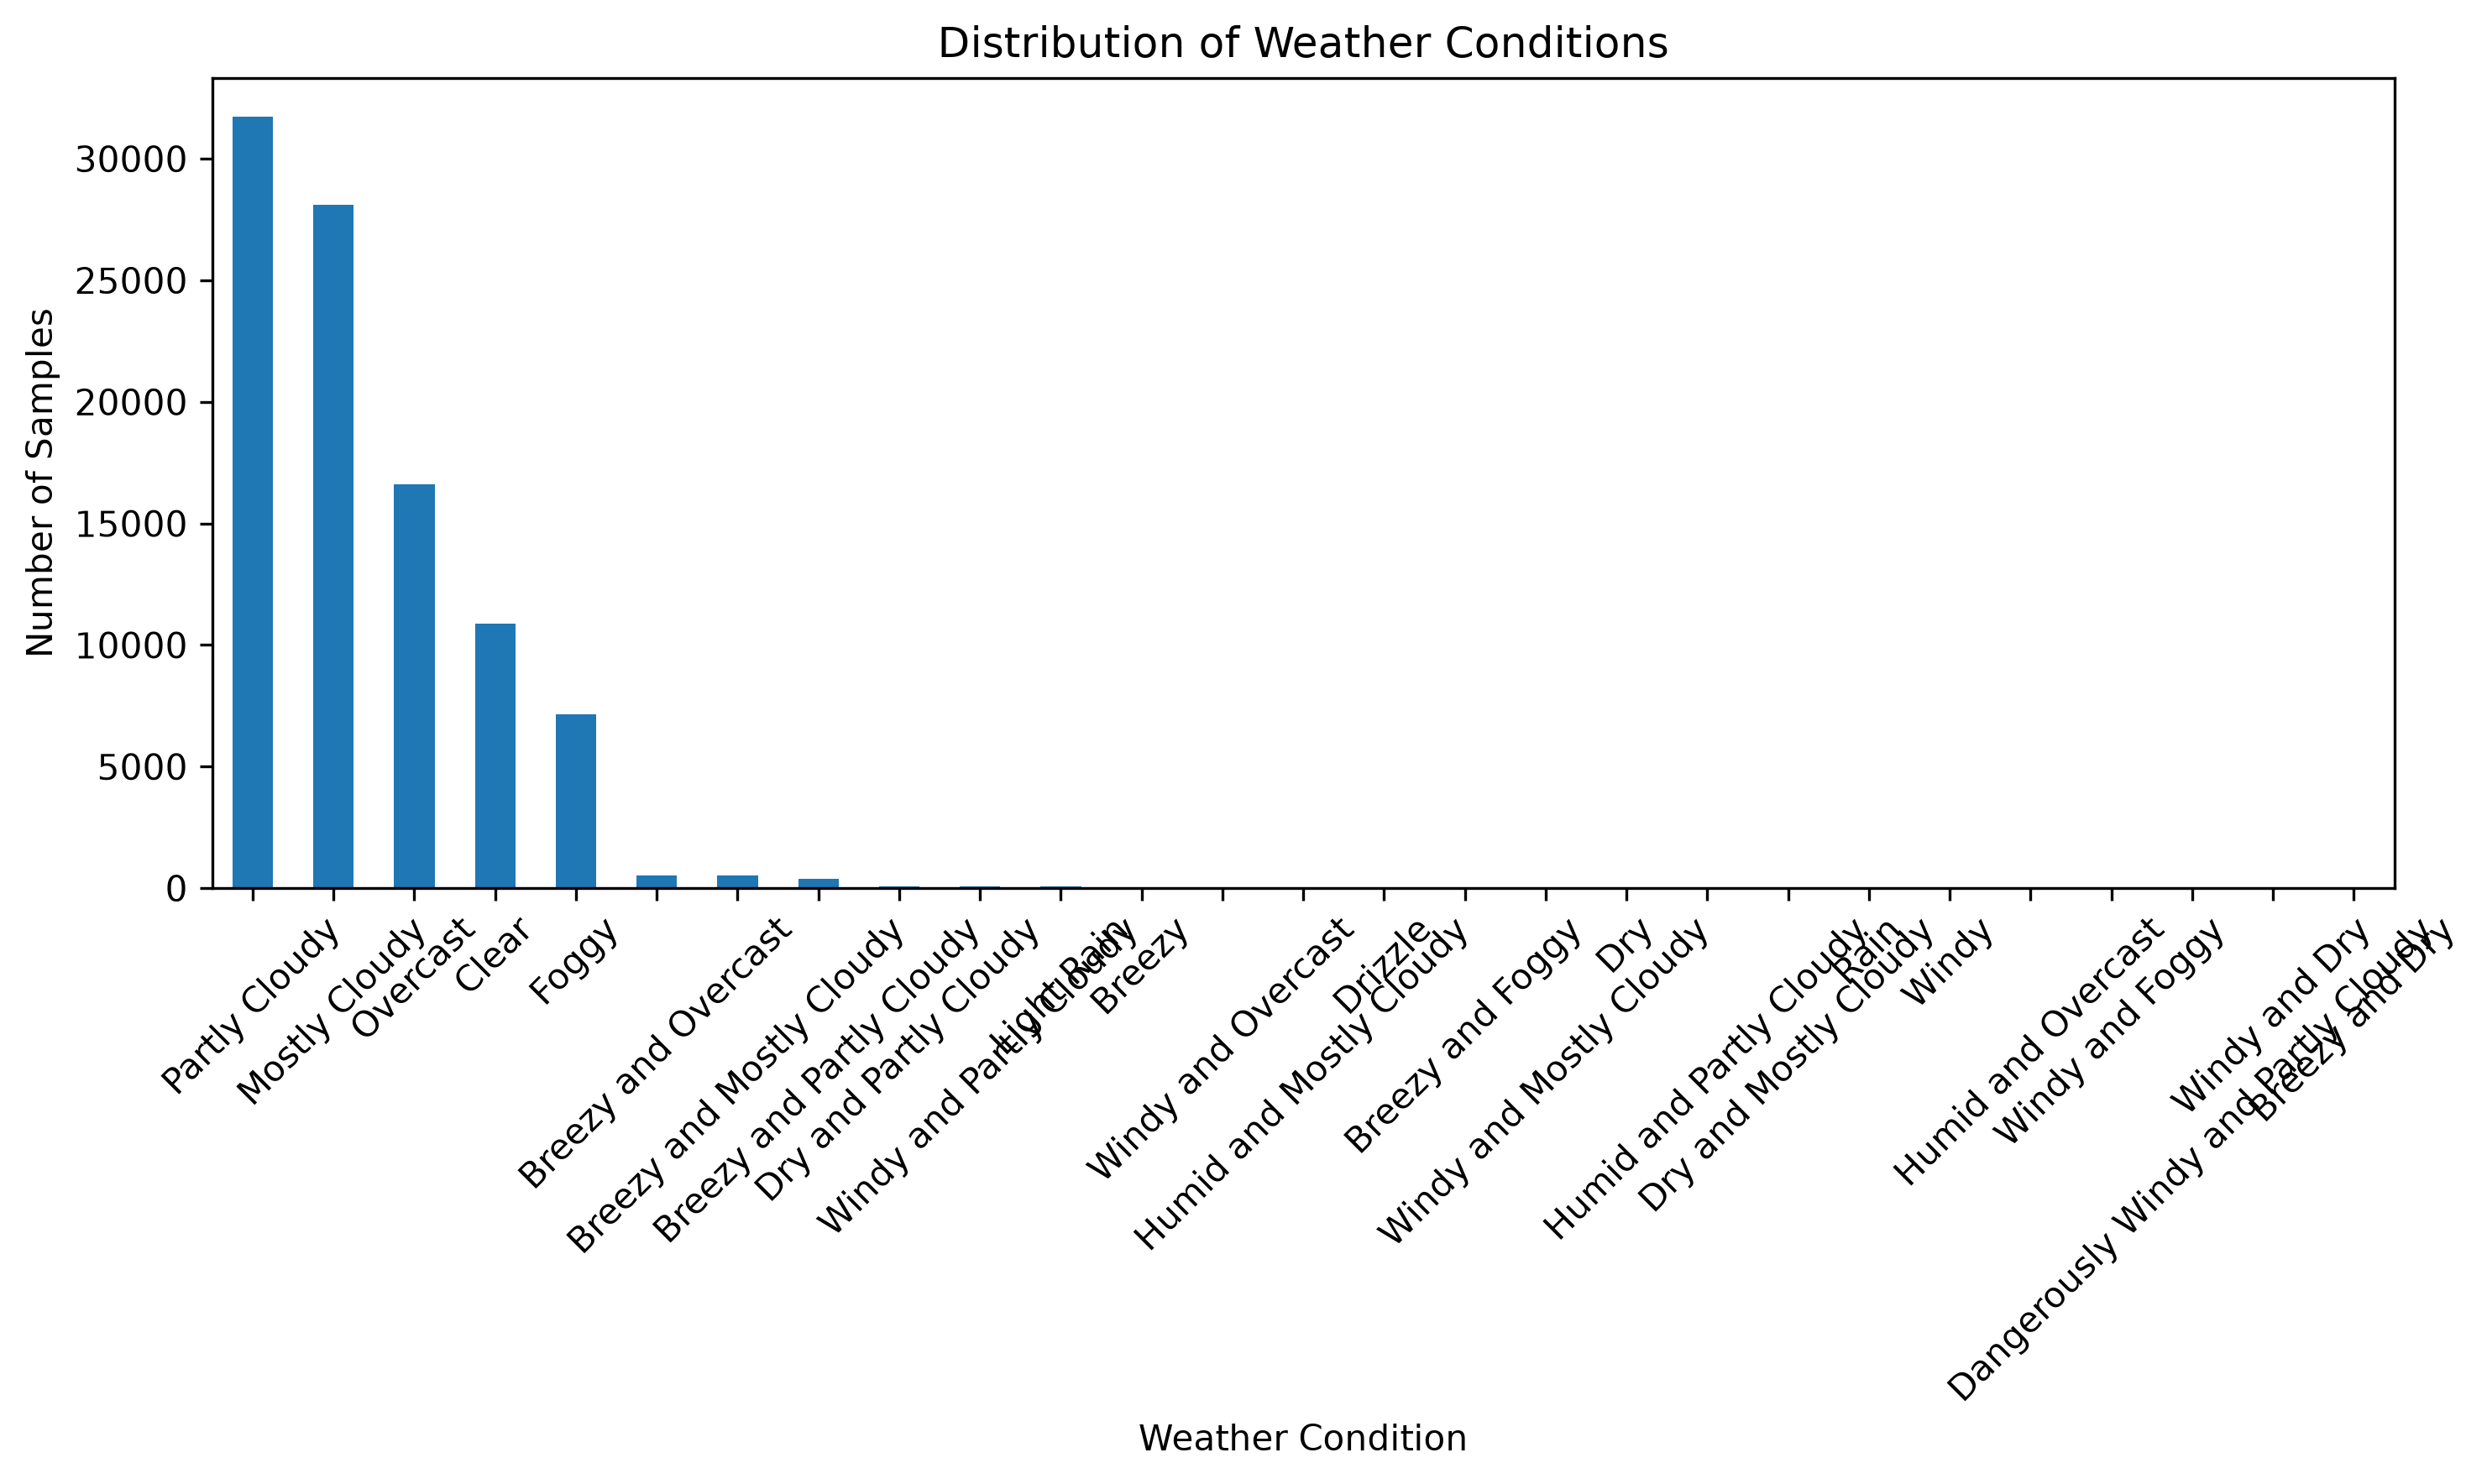
\includegraphics[width=\columnwidth]{figures/weather_distribution.png}
\caption{Class distribution in the processed weather dataset before rare-class filtering. The figure shows strong dominance by cloudy, overcast, clear, and foggy conditions, with a long tail of infrequent labels.}
\label{fig:distribution}
\end{figure}

The quantitative comparison is summarized in Table~\ref{tab:performance}. Random Forest achieved the highest weighted F1-score and was therefore selected as the best model. Fig.~\ref{fig:comparison} visually confirms the same ordering across the reported metrics.

\begin{table}[t]
\caption{PERFORMANCE COMPARISON OF CLASSIFICATION MODELS}
\label{tab:performance}
\centering
\begin{tabular}{>{\raggedright\arraybackslash}p{1.28in}cccc}
\toprule
Model & Acc. & Prec. & Rec. & F1 \\
\midrule
Logistic Regression & 0.5073 & 0.5004 & 0.5073 & 0.4832 \\
Decision Tree & 0.5799 & 0.5799 & 0.5799 & 0.5798 \\
Random Forest & 0.6215 & 0.6374 & 0.6215 & 0.6175 \\
\bottomrule
\end{tabular}
\end{table}


\begin{figure}[t]
\centering

\includegraphics[width=\columnwidth]{figures/model_comparison.png}
\caption{Comparison of accuracy, precision, recall, and weighted F1-score for the three evaluated classifiers. Random Forest leads all reported metrics, while Logistic Regression provides the weakest overall baseline.}
\label{fig:comparison}
\end{figure}

The weakest performer was Logistic Regression, with 0.5073 accuracy and 0.4832 weighted F1-score. Decision Tree improved the weighted F1-score to 0.5798, suggesting that nonlinear partitioning is more suitable than a purely linear boundary for this dataset. Random Forest further increased performance to 0.6215 accuracy, 0.6374 precision, 0.6215 recall, and 0.6175 weighted F1-score, indicating that an ensemble of trees captures broader interactions among meteorological variables.

\subsection{Confusion Matrix Analysis}
The confusion matrix for Random Forest is shown in Fig.~\ref{fig:cm}. The strongest large-support class is \textit{Foggy}, with 1{,}429 correct predictions out of 1{,}430 test examples. Strong recalls are also observed for \textit{Clear} (1{,}637/2{,}178), \textit{Overcast} (2{,}570/3{,}319), and several low-support windy or breezy variants after rare-class filtering.

\begin{figure}[t]
\centering
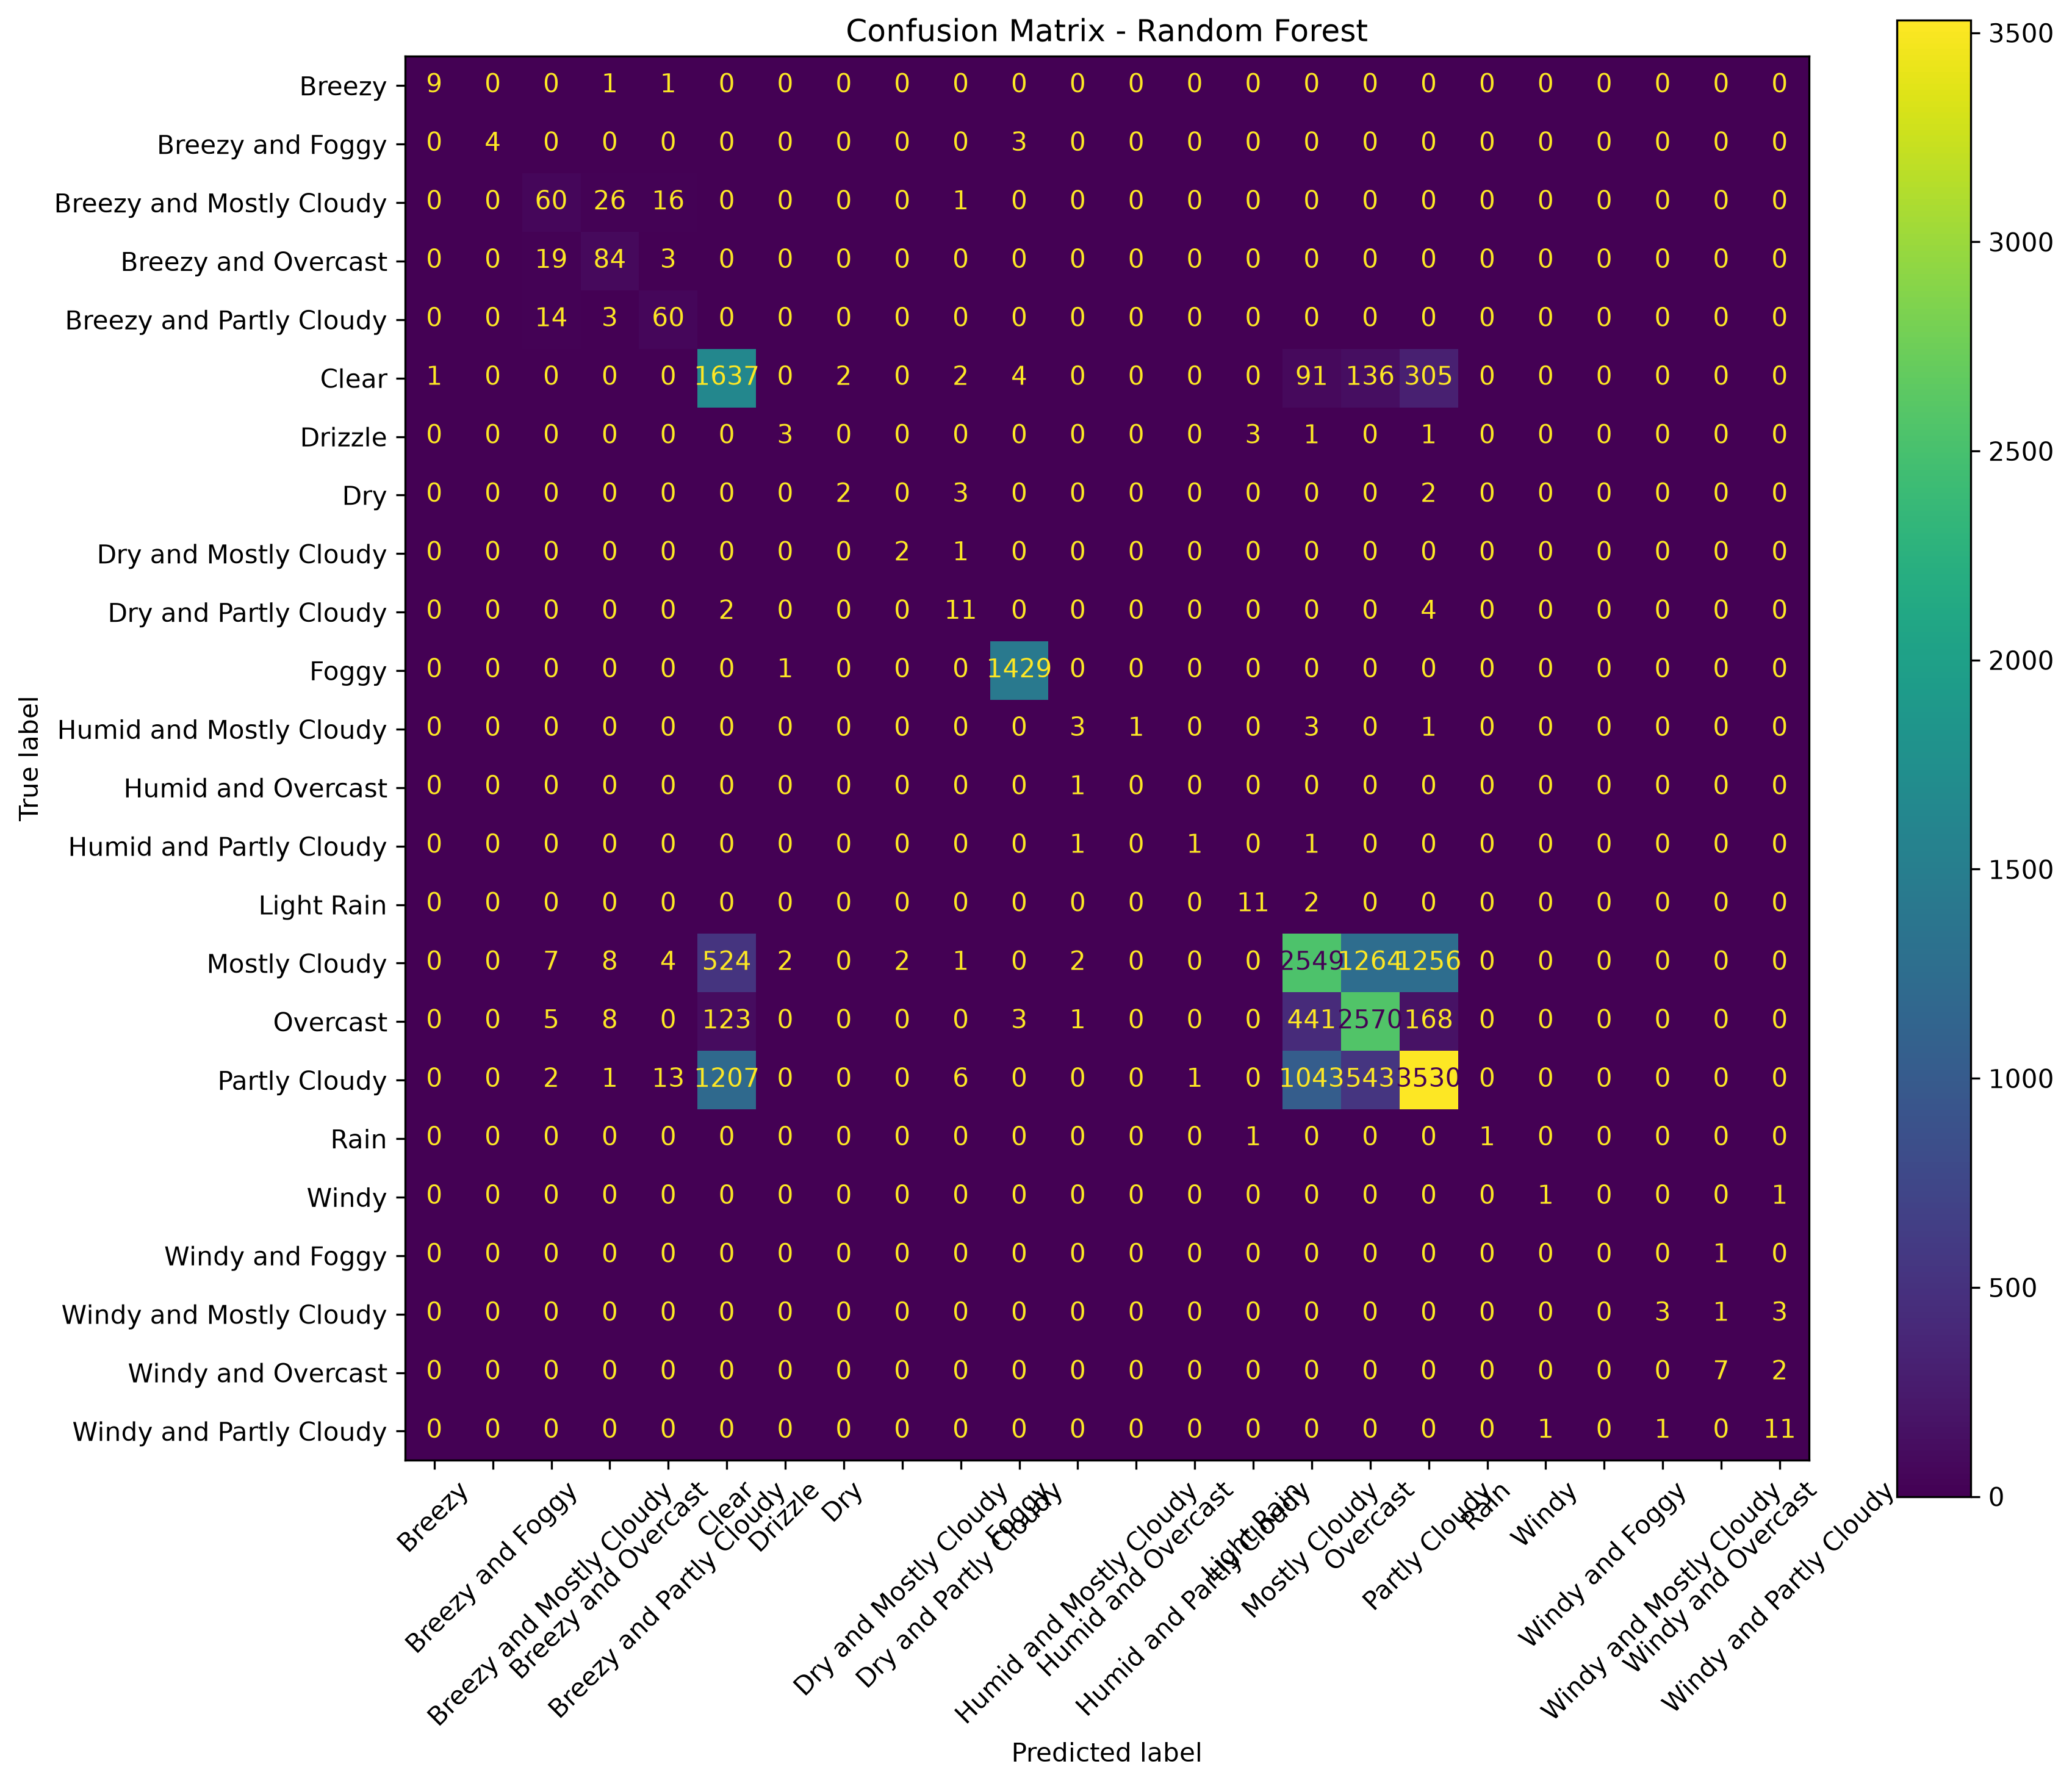
\includegraphics[width=\columnwidth]{figures/random_forest_confusion_matrix.png}
\caption{Random Forest confusion matrix on the stratified test set. Most large errors occur among semantically similar cloudy classes, especially \textit{Mostly Cloudy}, \textit{Overcast}, \textit{Partly Cloudy}, and \textit{Clear}.}
\label{fig:cm}
\end{figure}

The dominant errors occur among visually and meteorologically adjacent cloud-related labels. For example, \textit{Mostly Cloudy} is frequently predicted as \textit{Overcast} (1{,}264 cases) or \textit{Partly Cloudy} (1{,}256 cases). Likewise, \textit{Partly Cloudy} is often confused with \textit{Clear} (1{,}207 cases) and \textit{Mostly Cloudy} (1{,}043 cases). These patterns suggest genuine class overlap rather than isolated modeling failures. Minority classes such as \textit{Humid and Overcast} and \textit{Windy and Foggy} remain difficult because their support is extremely limited even after the rarest classes are removed.

\subsection{Feature Importance}
Random Forest feature importance is presented in Fig.~\ref{fig:importance}. The leading predictors are \textit{Wind Speed (km/h)} (0.1546), \textit{Humidity} (0.1170), \textit{Pressure (millibars)} (0.1058), \textit{Visibility (km)} (0.0986), \textit{Apparent Temperature (C)} (0.0910), and \textit{Temperature (C)} (0.0854).

\begin{figure}[t]
\centering
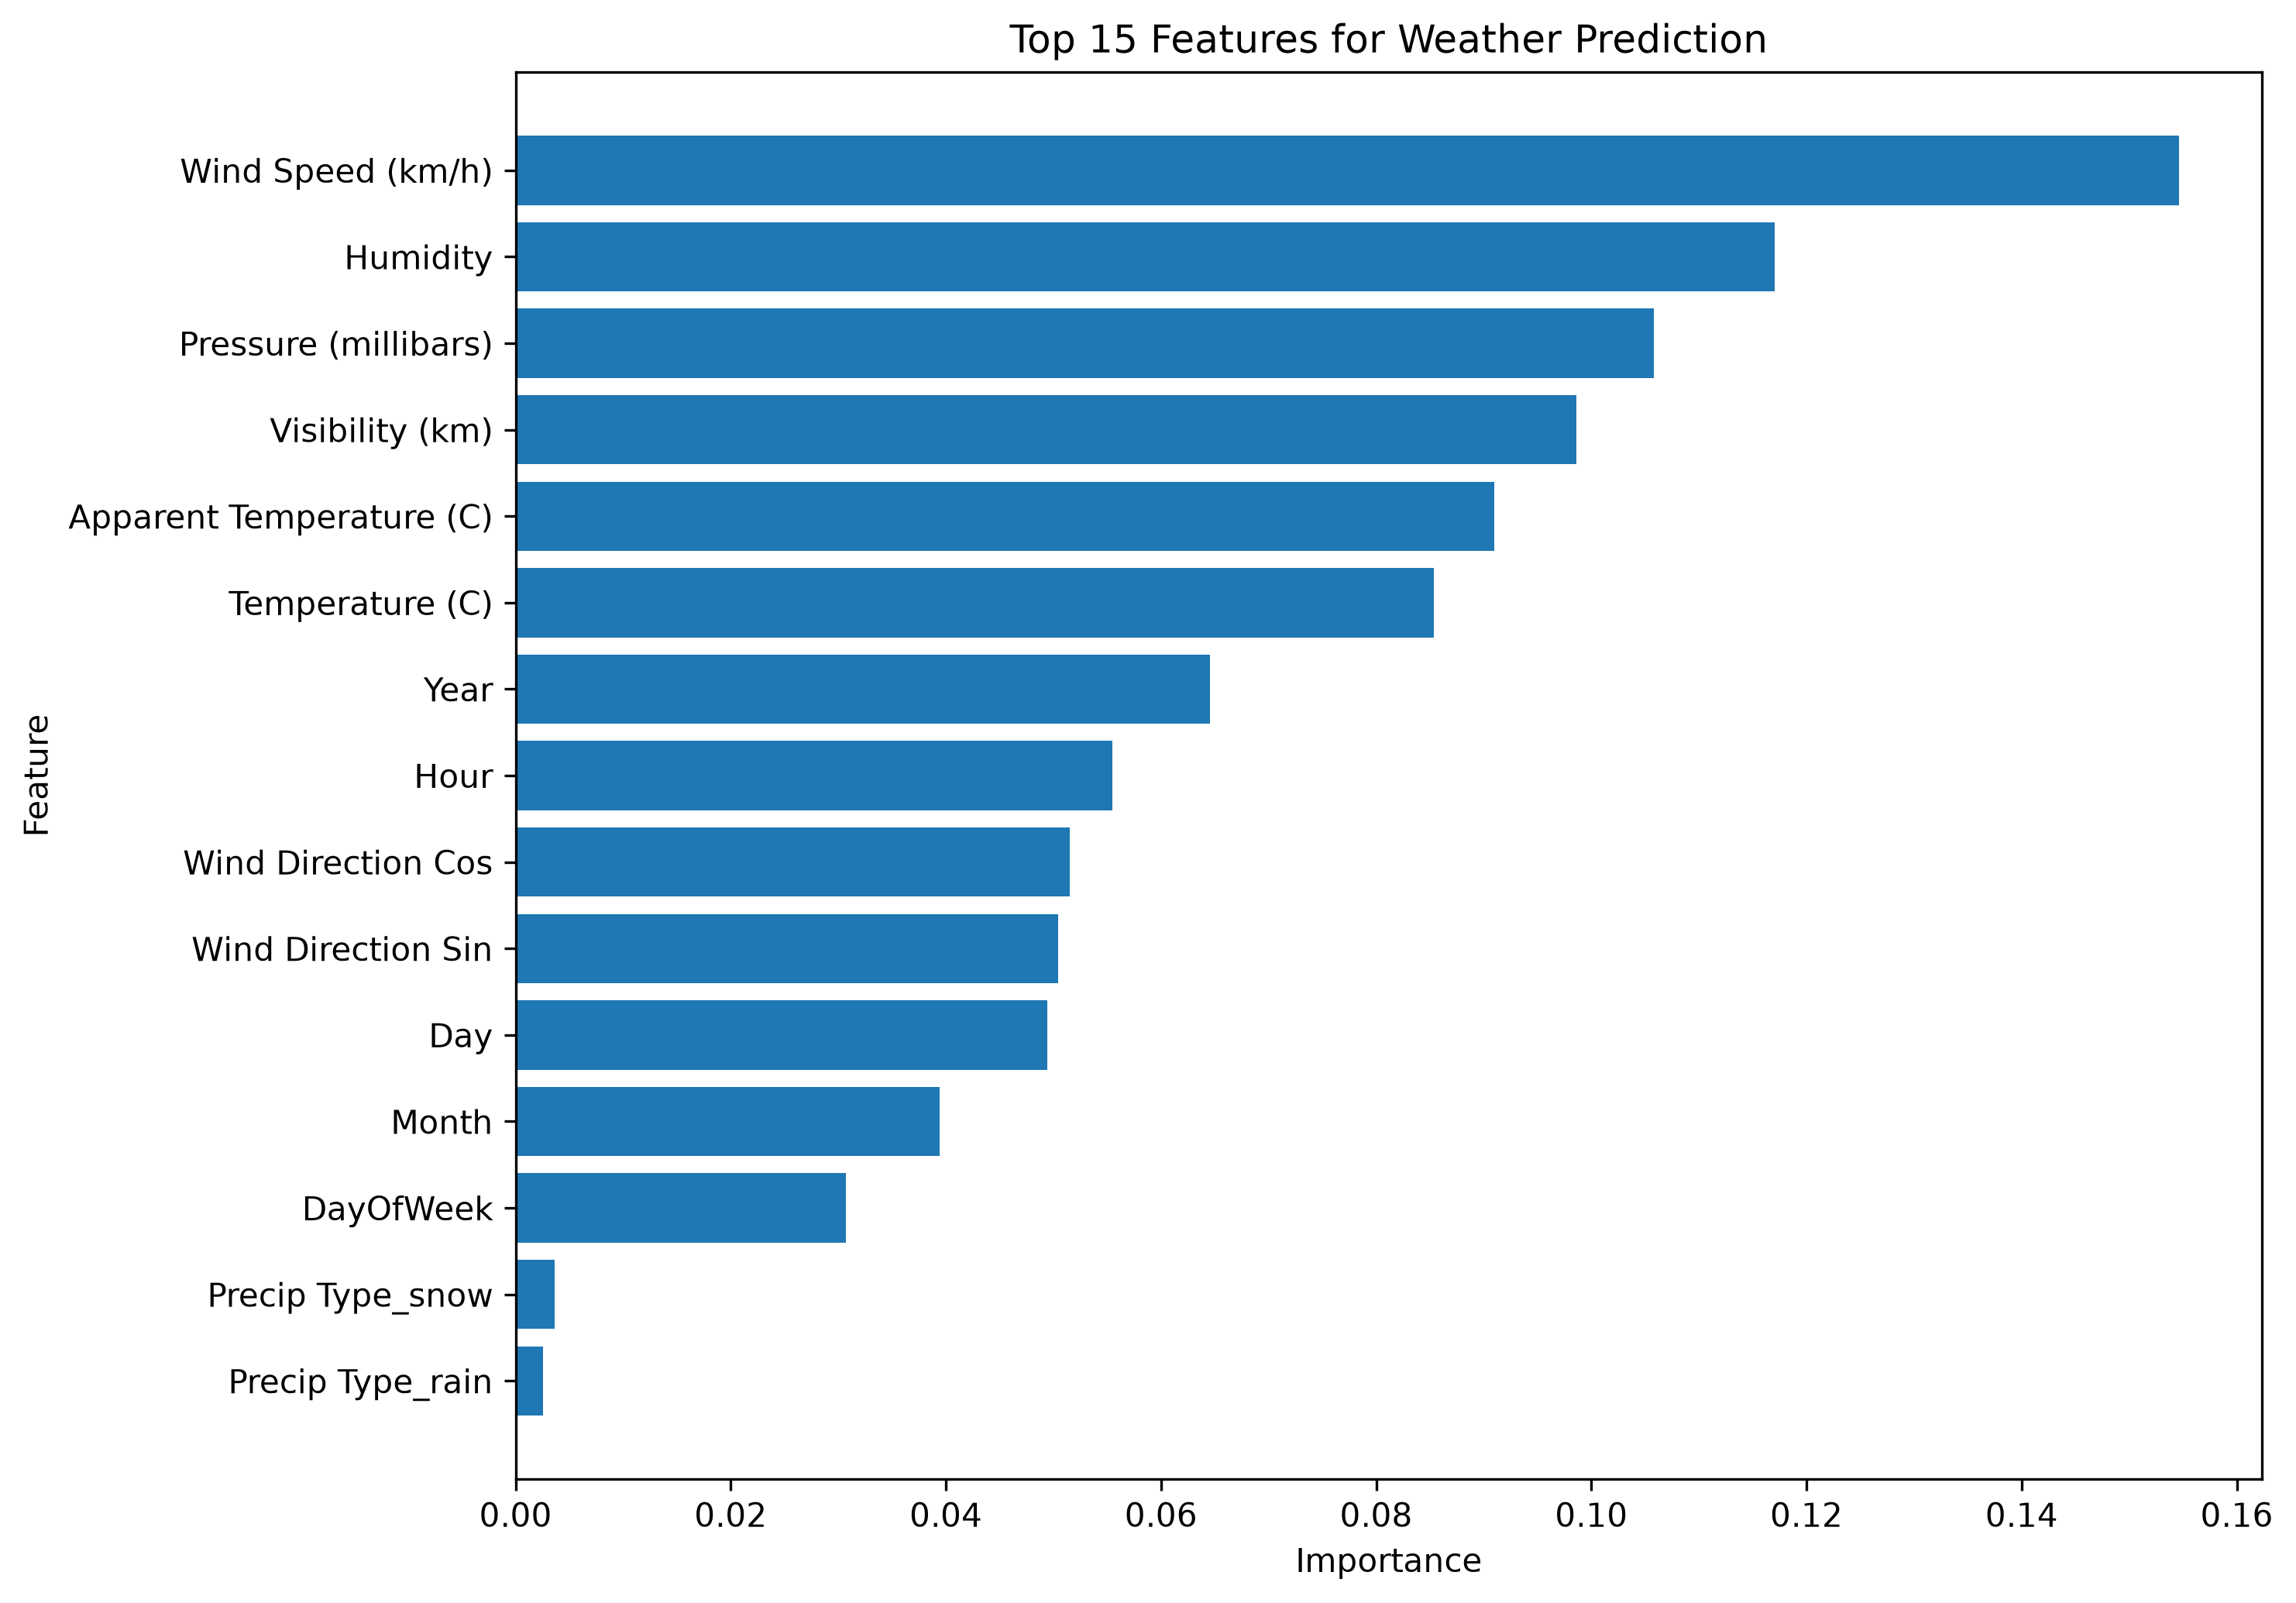
\includegraphics[width=\columnwidth]{figures/feature_importance.png}
\caption{Random Forest feature importance for the 15 model inputs. Wind speed, humidity, pressure, visibility, and temperature-related variables contribute most strongly to the classifier.}
\label{fig:importance}
\end{figure}

Temporal variables also contribute meaningfully, especially \textit{Year}, \textit{Hour}, \textit{Day}, and \textit{Month}, which indicates that weather-summary classes are partly structured by seasonal and diurnal context. The transformed circular wind features have moderate importance, validating the decision to encode directional information through sine and cosine components. By contrast, \textit{Precip Type\_rain} and \textit{Precip Type\_snow} have the smallest importance values in the saved model output, so precipitation type acts as a supplementary rather than dominant discriminator in this experiment.

\subsection{Comparative Analysis}
Taken together, the results show a consistent ranking: Random Forest $>$ Decision Tree $>$ Logistic Regression under weighted F1-score. The gap between Logistic Regression and the tree-based models suggests that the class boundaries are not well approximated by a linear classifier in the transformed feature space. The gap between Decision Tree and Random Forest indicates that averaging across many randomized trees improves robustness, particularly in the presence of noisy boundaries and imbalanced classes.




This study therefore has clear limitations. The findings are specific to one historical dataset and one target-labeling scheme. The model set is limited to three classical classifiers, and no external validation dataset was used. Rare weather conditions are underrepresented, and three one-sample classes had to be excluded before stratified evaluation. Accordingly, the results should be interpreted as a controlled comparative experiment on this dataset rather than evidence of operational real-time forecasting readiness.

\section{Conclusion}
This paper documented a complete multiclass weather-condition classification experiment based on the Kaggle Weather Dataset. The workflow removed non-informative fields, engineered temporal and circular wind-direction features, imputed missing values, one-hot encoded precipitation type, standardized numerical predictors, and preserved \textit{Summary} strictly as the prediction target to avoid leakage. After removing three one-sample classes, the study compared Logistic Regression, Decision Tree, and Random Forest under an 80/20 stratified split.

Among the evaluated models, Random Forest achieved the best recorded performance and was selected by weighted F1-score. Its test results were 0.6215 accuracy, 0.6374 precision, 0.6215 recall, and 0.6175 weighted F1-score. The confusion matrix and feature-importance outputs indicate that the classifier benefits most from wind speed, humidity, pressure, visibility, and temperature-related variables, while the main errors occur among semantically similar cloudy classes.

Future work may explore hyperparameter optimization, additional ensemble methods, temporal validation schemes, external weather datasets, and more explicit time-series modeling. These directions are proposed as future extensions, not as completed components of the current experiment.

\section*{About the Authors}
M. Komal Narasimha Rao is the primary author of this work.\
Roll No. 251LA18011\\
Email: komalnarashimharao@gmail.com

\balance
\bibliographystyle{IEEEtran}
\bibliography{references}

\end{document}
